\documentclass[border=4pt]{standalone}
\usepackage{amsmath,amssymb}
\usepackage{tikz}
\usetikzlibrary{arrows.meta}
\begin{document}
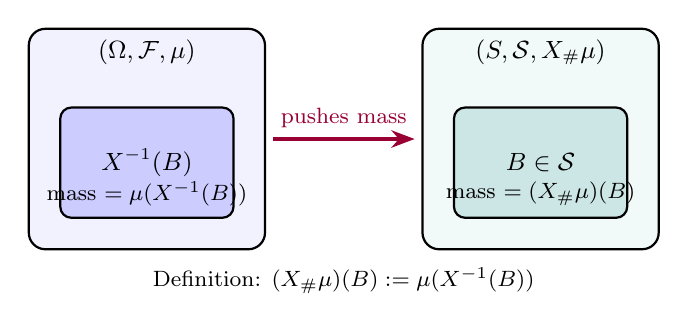
\begin{tikzpicture}[font=\small, >=Stealth]
  \draw[thick, fill=blue!5, rounded corners=6pt] (0,0) rectangle (3.0, 2.8);
  \node at (1.5, 2.5) {$(\Omega, \mathcal{F}, \mu)$};
  \draw[thick, fill=blue!20, rounded corners=4pt] (0.4, 0.4) rectangle (2.6, 1.8);
  \node at (1.5, 1.1) {$X^{-1}(B)$};
  \node[font=\footnotesize] at (1.5, 0.7) {mass $= \mu(X^{-1}(B))$};

  \draw[thick, fill=teal!5, rounded corners=6pt] (5.0,0) rectangle (8.0, 2.8);
  \node at (6.5, 2.5) {$(S, \mathcal{S}, X_\# \mu)$};
  \draw[thick, fill=teal!20, rounded corners=4pt] (5.4, 0.4) rectangle (7.6, 1.8);
  \node at (6.5, 1.1) {$B \in \mathcal{S}$};
  \node[font=\footnotesize] at (6.5, 0.7) {mass $= (X_\# \mu)(B)$};

  \draw[->, very thick, purple!80!black] (3.1, 1.4) -- node[above, font=\footnotesize] {pushes mass} (4.9, 1.4);
  \node[font=\footnotesize, align=center] at (4.0, -0.4) 
    {Definition: $(X_\# \mu)(B) := \mu(X^{-1}(B))$};
\end{tikzpicture}
\end{document}